\scanpage{94}
\figure{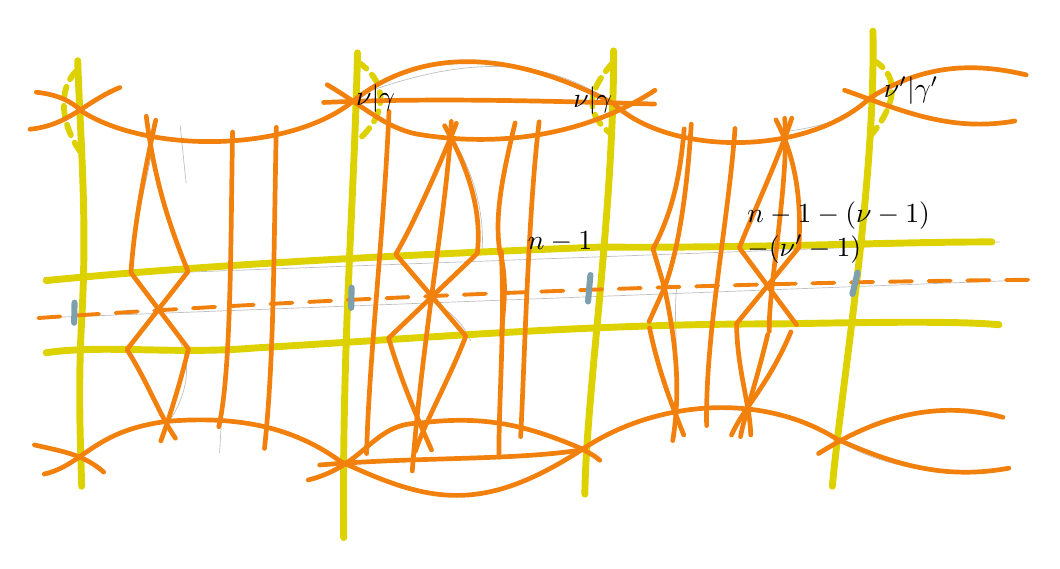
\begin{tikzpicture}[x=.005cm,y=-.005cm,line cap=round,line join=round]
\draw[gray!50,line width=.25pt] (275,790)--(2700,700) (257,893)--(2755,797) (500,780)..controls(500,620)and(560,495)..(550,400) (565,870)..controls(620,938)and(680,1020)..(590,1160) (620,405)--(635,550) (725,1150)--(720,1235) (1060,332)..controls(1340,226)and(1540,227)..(1718,347) (1300,422)..controls(1375,530)and(1394,650)..(1385,733) (1247,847)..controls(1308,872)and(1340,911)..(1357,950) (1880,816)..controls(1870,900)and(1889,1030)..(1877,1140) (2145,422)..controls(2250,406)and(2315,392)..(2377,332) (2300,1210)..controls(2410,1275)and(2590,1302)..(2728,1274);
\draw[yellow!70!olive,line width=2.5pt] (360,240)..controls(367,450)and(385,640)..(370,900)..controls(360,1080)and(368,1230)..(370,1320);
\draw[yellow!70!olive,line width=2.5pt] (1070,220)..controls(1062,590)and(1030,960)..(1035,1450);
\draw[yellow!70!olive,line width=2.5pt] (1720,215)..controls(1720,630)and(1650,1090)..(1647,1340);
\draw[yellow!70!olive,line width=2.5pt] (2378,165)..controls(2385,550)and(2300,1050)..(2275,1320);
\draw[yellow!70!olive,line width=2.5pt] (280,798)..controls(700,756)and(1250,730)..(1685,713)..controls(2080,716)and(2470,699)..(2680,700);
\draw[yellow!70!olive,line width=2.5pt] (280,981)..controls(425,960)and(610,986)..(810,969)..controls(1295,940)and(1690,907)..(2140,908)..controls(2400,903)and(2600,901)..(2698,910);
\draw[yellow!70!olive,dash pattern=on 4pt off 3pt,line width=2.1pt] (358,265)..controls(313,306)and(312,390)..(365,469);
\draw[yellow!70!olive,dash pattern=on 4pt off 3pt,line width=2.1pt] (1070,243)..controls(1135,283)and(1160,364)..(1070,443);
\draw[yellow!70!olive,dash pattern=on 4pt off 3pt,line width=2.1pt] (1718,245)..controls(1664,306)and(1638,365)..(1710,423);
\draw[yellow!70!olive,dash pattern=on 4pt off 3pt,line width=2.1pt] (2380,240)..controls(2453,281)and(2432,360)..(2370,433);
\draw[orange!80!brown,line width=1.7pt] (255,320)..controls(310,326)and(344,343)..(371,369)..controls(540,476)and(905,475)..(1066,337)..controls(1230,211)and(1450,207)..(1720,349)..controls(1860,482)and(2210,484)..(2370,335)..controls(2505,249)and(2634,244)..(2767,276);
\draw[orange!80!brown,line width=1.7pt] (239,414)..controls(340,403)and(375,346)..(467,308);
\draw[orange!80!brown,line width=1.7pt] (993,301)..controls(1085,355)and(1140,410)..(1220,426)..controls(1420,460)and(1643,434)..(1825,315);
\draw[orange!80!brown,line width=1.7pt] (984,346)..controls(1260,334)and(1540,342)..(1824,350);
\draw[orange!80!brown,line width=1.7pt] (2306,315)..controls(2440,362)and(2570,423)..(2738,393);
\draw[orange!80!brown,line width=1.7pt] (250,1215)..controls(318,1231)and(374,1238)..(426,1284);
\draw[orange!80!brown,line width=1.7pt] (275,1289)..controls(375,1266)and(400,1178)..(589,1155)..controls(770,1140)and(911,1172)..(1027,1257)..controls(1250,1361)and(1384,1393)..(1641,1226)..controls(1820,1105)and(2090,1077)..(2286,1200)..controls(2430,1265)and(2560,1304)..(2723,1274);
\draw[orange!80!brown,line width=1.7pt] (945,1304)..controls(1090,1268)and(1108,1161)..(1225,1160)..controls(1400,1137)and(1510,1170)..(1640,1225)..controls(1660,1237)and(1670,1241)..(1685,1254);
\draw[orange!80!brown,line width=1.7pt] (974,1266)..controls(1220,1245)and(1470,1255)..(1643,1227);
\draw[orange!80!brown,line width=1.7pt] (2240,1237)..controls(2377,1150)and(2530,1098)..(2708,1145);
\draw[orange!80!brown,line width=1.7pt] (534,381)..controls(554,536)and(587,645)..(640,775)--(485,973)..controls(540,1060)and(568,1140)..(608,1198);
\draw[orange!80!brown,line width=1.7pt] (558,391)..controls(521,560)and(503,668)..(495,778)--(641,971)..controls(620,1060)and(591,1150)..(571,1205);
\draw[orange!80!brown,line width=1.7pt] (753,421)..controls(748,688)and(750,1030)..(718,1169);
\draw[orange!80!brown,line width=1.7pt] (864,409)..controls(857,727)and(859,988)..(834,1224);
\draw[orange!80!brown,line width=1.7pt] (1150,369)..controls(1136,685)and(1100,987)..(1093,1237);
\draw[orange!80!brown,line width=1.7pt] (1291,405)..controls(1325,467)and(1390,591)..(1374,729)--(1149,944)..controls(1183,1060)and(1226,1156)..(1258,1228);
\draw[orange!80!brown,line width=1.7pt] (1321,399)..controls(1281,500)and(1207,665)..(1167,731)--(1345,939)..controls(1302,1050)and(1240,1160)..(1217,1231);
\draw[orange!80!brown,line width=1.7pt] (1308,394)..controls(1299,600)and(1235,938)..(1209,1281);
\draw[orange!80!brown,line width=1.7pt] (1470,398)..controls(1432,555)and(1419,640)..(1431,724)..controls(1454,810)and(1437,877)..(1436,938);
\draw[orange!80!brown,line width=1.7pt] (1435,724)..controls(1444,930)and(1428,1100)..(1429,1246);
\draw[orange!80!brown,line width=1.7pt] (1531,395)..controls(1503,621)and(1493,1030)..(1484,1194);
\draw[orange!80!brown,line width=1.7pt] (1899,413)..controls(1889,530)and(1871,620)..(1820,718)--(1849,816)..controls(1880,963)and(1890,1079)..(1870,1204);
\draw[orange!80!brown,line width=1.7pt] (1917,401)..controls(1906,577)and(1884,723)..(1849,816)--(1810,902);
\draw[orange!80!brown,line width=1.7pt] (1811,918)..controls(1834,1027)and(1864,1105)..(1898,1190);
\draw[orange!80!brown,line width=1.7pt] (2028,412)..controls(2011,648)and(1952,935)..(1956,1166);
\draw[orange!80!brown,line width=1.7pt] (2132,390)..controls(2191,504)and(2195,618)..(2190,714)--(2032,907)..controls(2033,1023)and(2066,1112)..(2068,1190);
\draw[orange!80!brown,line width=1.7pt] (2172,386)..controls(2135,498)and(2063,651)..(2039,715)--(2184,910);
\draw[orange!80!brown,line width=1.7pt] (2170,928)..controls(2112,1065)and(2050,1120)..(2019,1190);
\draw[orange!80!brown,line width=1.7pt] (2154,386)..controls(2167,536)and(2111,828)..(2115,927);
\draw[orange!80!brown,line width=1.7pt] (2111,935)..controls(2081,1060)and(2051,1144)..(2042,1194);
\draw[orange!80!brown,line width=1.4pt,dash pattern=on 8pt off 6pt] (260,893)..controls(1100,835)and(2050,802)..(2777,796);
\draw[cyan!30!gray,line width=2.2pt] (352,854)--(351,905) (1055,816)--(1054,867) (1661,784)--(1655,851) (2339,778)--(2326,832);
\node at (1116,337) {$\unsure{\nu|\gamma}$};\node at (1667,340) {$\unsure{\nu|\gamma}$};\node at (2475,316) {$\unsure{\nu'|\gamma'}$};
\node at (1584,699) {$n-1$};\node[align=left] at (2291,676) {$n-1-(\nu-1)$\\$-(\nu'-1)$};
\end{tikzpicture}}
% crop-candidate: scan 94

Version du \unsure{raccordement} supersingulier
adapté à l'étude de l'application $\mathcal X-X$,
mais non \deleted{\unsure{aux}} \deleted{\unsure{dans la}} structures
$2n$-gonales des faces et à l'étude
du transport parallèle de celles-ci.
Dans l'autre version, on aplatit la
bande supersingulière sur son axe
central (pointillé rouge). Le transport
parallèle \inserted{(de franchissement d'une position supersingulière)} n'est \uline{pas} celui donné
par l'identification des côtés \unsure{utilisée|utilisé}
pour construire $\mathcal X$, mais est l'anti-
podique de celui-ci. La
relation entre transport parallèle \inserted{$\tau_X$} sur
$X$, et transport-réflexions \inserted{$\tau_{\mathcal X}$} sur $\mathcal X$,
pour un chemin donné sur $\mathcal X$, est
\deleted{\unsure{qu'ils sont de}} $\tau_X=\uline{a}^{\nu}\tau_{\mathcal X}$,
où $a$ est l'antipodisme, et $\nu$ le nb.
de franchissements d'une ligne
de superrégularité. Les deux syst. locaux associés
\unsure{sur $\widetilde{\mathcal X}$} \illegible{3} \unsure{donc connexes} \unsure{les deux}
\margin{93}
